\section{数据库}

\subsection{生物信息学数据库的分类}

生物信息学常见数据库如\autoref{tab:生物信息学常见数据库}所示。

\begin{table}[htbp]
	\begin{tabularx}{\textwidth}{|cc|X|}
		\hline
		\multicolumn{2}{|c|}{分类} & \multicolumn{1}{c|}{名称} \\ \hline
		\multicolumn{1}{|c|}{\multirow{2}{*}{核酸数据库}} & 一级 & GenBank、EMBL、DDBJ(同属于INSDC) \\ \cline{2-3}
		\multicolumn{1}{|c|}{} & 二级 & RefSeq、dbEST、Gene(同属于NCBI) \\ \hline
		\multicolumn{1}{|c|}{\multirow{3}{*}{蛋白质数据库}} & 一级,序列 & SWISSPROT、TrEMBL、PIR(同属于UniProt) \\ \cline{2-3}
		\multicolumn{1}{|c|}{} & 一级,结构 & PDB \\ \cline{2-3}
		\multicolumn{1}{|c|}{} & 二级 & SCOP、CATH、STRING等 \\ \hline
		\multicolumn{1}{|c|}{专用数据库} &  & OMIM、PubMed、ZINC、KEGG \\ \hline
	\end{tabularx}
	\caption{生物信息学常见数据库}
	\label{tab:生物信息学常见数据库}
\end{table}

\subsection{一级核酸数据库}

主要包括三大核酸数据库和基因组数据库。

三大核酸数据库分别是:

\begin{description}
	\item[GenBank] 由NCBI(National Center for Biotechnology Information)创建和维护。
	\item[ENA(European Nucleotide Archive)] 由EMBL(European Molecular Biology Laboratory)开发并维护。
	\item[DDBJ(DNA Data Bank of Japan)] 由NIG(National Institute of Genetics)开发并维护。
\end{description}
以上三者合称INSDC(International Nucleotide Sequence Database)。

两个基因组数据库分别是:
\begin{description}
	\item[Ensemble] 收录了各种动物的基因组,尤其是与人类亲缘关系近的。注释是软件自动添加的。
	\item[Phytozome] 收录了植物的基因组,缺点是裸子植物比较少,因为其转座子多。
\end{description}

\subsubsection{GenBank}

登录\href{https://www.ncbi.nlm.nih.gov/genbank/}{GenBank},进入一个条目(以\href{https://www.ncbi.nlm.nih.gov/nuccore/X01714}{X01714}为例,\autoref{fig:genbankx01714}和\autoref{chapter:GenbankX01714})。

\begin{figure}[htbp]
	\centering
	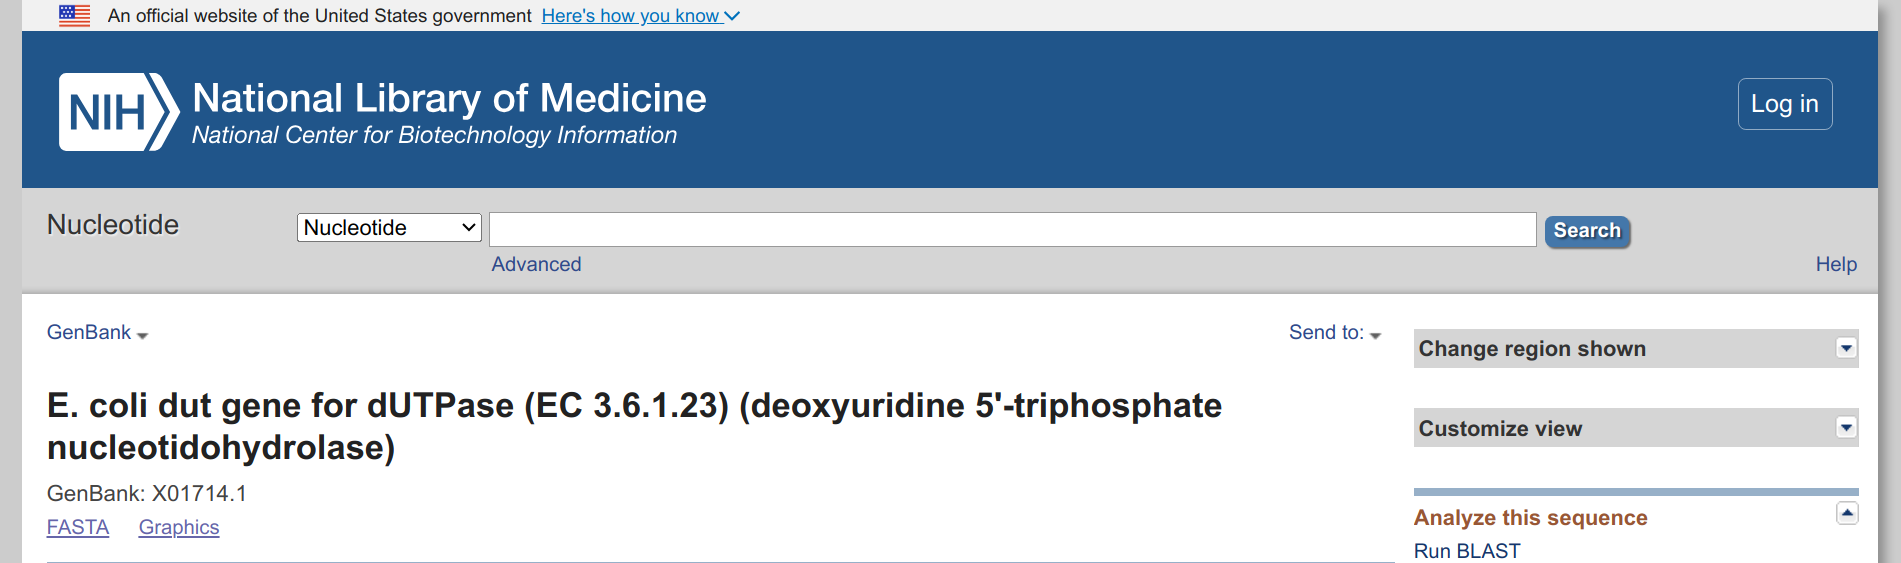
\includegraphics[width=\textwidth]{Genbank_X01715.png}
	\caption{GenBank, X01714}
	\label{fig:genbankx01714}
\end{figure}

在页面显示的信息中,下面几个较为重要:

\begin{description}
	\item[基因真名\texttt{LOCUS}] 研究者给这个基因取的名字,有时会与检索号\texttt{ACCESSION}相同(如本例),但也可不同。本例,LOCUS为X01714。
	\item[碱基数、基因类别、拓扑类型、上传日期] 按顺序,都位于第一行。需要注意,来自细菌(Bacteria)的数据会加上\texttt{BCT}字样(如本例)。
	\item[检索号\texttt{ACCESSION}] 相当于基因的身份证号,一旦发布,不再修改。
	\item[版本\texttt{VERSION}] 若测序有误或是其他原因使得序列有更新,则版本号会变动。
	\item[特点\texttt{FEATURES}] 描述了该基因的信息,含有许多子条目。需要注意,其中的\texttt{/translation=}部分的氨基酸序列为计算机自动生成,并非实验测得。
	\item[序列\texttt{ORIGIN}] 记录了该基因的序列,以\texttt{//}标识序列结束。
\end{description}

在查询时,若遇到条目后一个\texttt{.}的情况,这是数据缺失的意思。所有的数据库都存在数据不完整的问题。

\subsubsection{基因组数据库}

如前所述,基因组数据库主要有动物的Ensemble和植物的Phytozome。

\subsection{二级核酸数据库}

常用的是NCBI下属的三个数据库:
\begin{description}
	\item[RefSeq] 通过自动和人工精选出的非冗余数据库,不仅包含核酸序列,也包含蛋白质序列。凡是名字里有ref的都是去冗余数据库,即去掉了重复的内容。
	\item[dbEST] EST即表达序列标签,存储的是不同物种的EST,即cDNA。
	\item[Gene] 以基因为记录对象,提供基因序列的检索和注释。
\end{description}

其他二级核酸数据库还有ncRNAdb(非编码RNA数据库)、miRBase(microRNA数据库)等。

\subsection{一级蛋白质数据库}

包括UniProt的三个组成部分:
\begin{description}
	\item[Swiss-Prot] 人工注释,因此注释可信度高,冗余量小。
	\item[TrEMBL] 包含所有从EMBL由计算机翻译而来的蛋白质,Tr-意即translation。蛋白质序列注释由计算机完成,故可信度低,冗余多。
	\item[PIR] 中文名是蛋白质信息资源数据库。
\end{description}

由于序列的来源不一样,故Swiss-Prot比TrEMBL小得多。

\subsubsection{UniProt}

\href{https://www.uniprot.org/}{UniProt数据库}分为三个层次:

\begin{description}
	\item [第一层:UniParc] 意为UniProt Archieve,收录了三个子数据库中的全部序列。
	\item[第二层:UniRef] 去冗余后的数据库。
	\item[第三层:UniProtKB] 意为UniProt Knowledge Base,有详细注释,与其他数据库有链接。
\end{description}

UniProt网站上提供的信息有:

\begin{description}
	\item [基本信息]物种、基因名称等。
	\item [功能]催化的反应、杂项。
	\item [名称、谱系]所属物种的谱系、蛋白质本身的全名、缩写、别名。
	\item [亚细胞定位] 提供亚细胞定位的蛋白质多数来源于Swiss-Prot。
	\item[疾病、变种] 提供蛋白质变异后引发的疾病。
	\item[转录后加工]
	\item[表达水平] 包括mRNA、细胞中、不同组织中的表达水平。
	\item[相互作用] 提供蛋白质相互作用信息。
	\item[结构] 数据来源于PDB。
	\item[家族、结构域]
	\item[序列、异构体] 含多个异构体的蛋白质会显示多条序列。
	\item[相似蛋白质] 提供从UniRef数据库中找到的在一级结构上相似的蛋白质。
\end{description}

\subsubsection{PDB}

PDB数据库是唯一储存生物大分子三维结构的数据库,除了蛋白质以外,还包括核酸和核酸与蛋白质的复合物。但是只有通过实验方法得到的数据才会被收录。

PDB中,每个蛋白质都有一个四字节的序号,如\texttt{5RJM},其中第一位永远是数字,后面三位是大写字母和数字的组合。

\subsection{二级蛋白质数据库}

\subsubsection{Pfam}

Pfam收录蛋白质的结构域。

\subsubsection{CATH}

CATH对蛋白质的结构域,按照结构特征进行了分类,分为Class、Architecture、Topology、Homologous Superfamily四个层次。

\subsubsection{SCOP2}

与CATH相似,但是其分类原则更侧重蛋白质的进化关系,而且分类主要依赖于人工验证。四个层次分别是:Class、Fold、Superfamily、Family。

\subsection{专用数据库}

\subsubsection{PubMed}

\href{https://pubmed.ncbi.nlm.nih.gov/}{PubMed}是一个文献数据库,收录了最早至1965年的许多生物医学文献。要点有:

\begin{itemize}
	\item 搜索到的每篇文献都有一个唯一的PubMed ID(PMID);
	\item 提供指向文献的链接,但是否能够阅读取决于你的网络(如校园网);
	\item PubMed并没有收录全部与生物医学有关的文献(想想也不可能)。
\end{itemize}

\subsubsection{OMIM}

\href{https://www.omim.org/}{OMIM(Online Mendelian Inheritance in Man)},中文翻译为“人类孟德尔遗传在线”,存储了大量已知的孟德尔遗传病的相关信息。

\subsubsection{KEGG}

\href{https://www.genome.jp/kegg/}{KEGG(Kyoto Encyclopedia of Genes and Genomes)},存储了生物体内的代谢通路信息。

\subsubsection{ZINC}

\href{https://zinc.docking.org/}{ZINC}存储有机小分子的三维结构信息,主要用于药物发现中的虚拟筛选。

\section{序列比对}

\subsection{FASTA格式}

FASTA格式是蛋白质或核酸序列的一种通用书写格式。要点有:
\begin{itemize}
	\item 第一行开头是大于号,之后跟随名称或者其他注释;
	\item 后面几行,每行60个字母,最后一行除外,但要求并不是很严格。
\end{itemize}

下面是一个实例,其中\texttt{Q9UNS1}是该序列在UniProt中的编号:

\begin{verbatim}
		>sp|Q9UNS1|
		MDLHMMNCELLATCSALGYLEGDTYHKEPDCLESVKDLIRYLRHEDETRDVRQQLGAAQI
		LQSDLLPILTQHHQDKPLFDAVIRLMVNLTQPALLCFGNLPKEPSFRHHFLQVLTYLQAY
		KEAFASEKAFGVLSETLYELLQLGWEERQEEDNLLIERILLLVRNILHVPADLDQEKKID
		DDASAHDQLLWAIHLSGLDDLLLFLASSSAEEQWSLHVLEIVSLMFRDQNPEQLAGVGQG
		RLAQERSADFAELEVLRQREMAEKKTRALQRGNRHSRFGGSYIVQGLKSIGERDLIFHKG
		LHNLRNYSSDLGKQPKKVPKRRQAARELSIQRRSALNVRLFLRDFCSEFLENCYNRLMGS
		VKDHLLREKAQQHDETYYMWALAFFMAFNRAASFRPGLVSETLSVRTFHFIEQNLTNYYE
		MMLTDRKEAASWARRMHLALKAYQELLATVNEMDISPDEAVRESSRIIKNNIFYVMEYRE
		LFLALFRKFDERCQPRSFLRDLVETTHLFLKMLERFCRSRGNLVVQNKQKKRRKKKKKVL
		DQAIVSGNVPSSPEEVEAVWPALAEQLQCCAQNSELSMDSVVPFDAASEVPVEEQRAEAM
		VRIQDCLLAGQAPQALTLLRSAREVWPEGDVFGSQDISPEEEIQLLKQILSAPLPRQQGP
		EERGAEEEEEEEEEEEEELQVVQVSEKEFNFLDYLKRFACSTVVRAYVLLLRSYQQNSAH
		TNHCIVKMLHRLAHDLKMEALLFQLSVFCLFNRLLSDPAAGAYKELVTFAKYILGKFFAL
		AAVNQKAFVELLFWKNTAVVREMTEGYGSLDDRSSSRRAPTWSPEEEAHLRELYLANKDV
		EGQDVVEAILAHLNTVPRTRKQIIHHLVQMGLADSVKDFQRKGTHIVLWTGDQELELQRL
		FEEFRDSDDVLGHIMKNITAKRSRARIVDKLLALGLVAERRELYKKRQKKLASSILPNGA
		ESLKDFCQEDLEEEENLPEEDSEEEEEGGSEAEQVQGSLVLSNENLGQSLHQEGFSIPLL
		WLQNCLIRAADDREEDGCSQAVPLVPLTEENEEAMENEQFQQLLRKLGVRPPASGQETFW
		RIPAKLSPTQLRRAAASLSQPEEEQKLQPELQPKVPGEQGSDEEHCKEHRAQALRALLLA
		HKKKAGLASPEEEDAVGKEPLKAAPKKRQLLDSDEEQEEDEGRNRAPELGAPGIQKKKRY
		QIEDDEDD
\end{verbatim}

\subsection{序列相似性分析}

\subsubsection{替换记分矩阵}

反映残基之间相互替换率的矩阵,量化了核酸或氨基酸残基之间的相似性。分为核酸和蛋白质两类。

\paragraph{DNA序列的替换计分矩阵}

有等价矩阵、转换-颠换矩阵、BLAST矩阵三种。

\begin{description}
	\item[等价矩阵] 碱基相同记1分,不同记0分,过于简单,应用很少。
	\item[转换-颠换矩阵] 碱基转换比颠换容易,故转换的得分比颠换高。也很少用。
	\item[BLAST矩阵] 相同记+5分,不同记-4分。应用广泛,效果最好。
\end{description}


\paragraph{蛋白质序列的替换记分矩阵}

有等价矩阵、遗传密码矩阵、疏水性矩阵、PAM矩阵、BLOSUM矩阵。

\begin{description}
	\item[等价矩阵] 同DNA。
	\item[遗传密码矩阵] 考虑发生氨基酸变化所需密码子变化数目,常用于演化距离的计算,而不是序列比对。
	\item[疏水性矩阵] 考虑氨基酸替换后理化性质的改变,适用于偏功能方面的比对。
	\item[PAM矩阵] 演化历史上,频繁发生替换的氨基酸得分较高,PAM-1矩阵表示平均每100个氨基酸发生一个突变时,各个氨基酸发生替换的得分。自乘n次得到PAM-n。
	\item[BLOSUM矩阵] BLOSUM矩阵的编号(如80)就是构建这个矩阵时,把相似度超过这个百分比的序列合并为一类,避免过多侧重高相似度的统计数据\footnote{因为这样会让保守的氨基酸替换得很高的分数。}。
\end{description}

在PAM和BLOSUM矩阵中,对角线上的数值代表相同氨基酸的得分,而且并不完全相同,其他位置得分大于0则相似,小于0则不相似。

选择PAM还是BLOSUM的原则是:
\begin{itemize}
	\item 序列相似度越高,应选择的BLOSUM数值越高,PAM数值越低;
	\item 未知序列相似度时,先用BLOSUM62试一试;
\end{itemize}

\subsubsection{比较序列的方法}

\paragraph{打点法}

把要比较的两条序列,一条横着写,另一条竖着写,相同字母就做上记号,比较的次数是两条序列长度乘积。

连续的对角线和其平行线代表两条序列中相同的区域,有助于发现短串联重复序列(STR)。

\paragraph{序列比较法}

运用算法找出两个或多个序列之间产生最大相似度得分的空格插入、字母替换的方案。这需要用到前面的替换计分矩阵。常用的算法是Needleman-Wunch算法。

\subparagraph{双序列全局比对}



两条序列插GAP,得分要最高。

全局比对global alignment:Needleman-Wunsch算法 用于比较两条长度相似的序列

一致度indentity 相似度similarity

gap open 扣多少分  gap extend每个扣多少分

若gap open扣分比gap extend多,

|上下一致 :上下相似 .上下不相似 短横- 空位

局部比对local alignment
也是N-W二人发明的算法

全局比对有时会抹杀了两条序列在局部上的相似度,而这是很有生物学意义的。

使用局部比对工具

多序列比对

\begin{itemize}
	\item 太多的序列受不了。不要超过50条。
	\item 关系太远的序列受不了。两两之间序列相似度低于30\%的一组序列,作多序列比对会有麻烦。
	\item 关系太近的序列受不了。两两之间序列相似度大于90\%的序列,有再多条都等于只有一条。
	\item 短序列受不了。多序列比对支持一组差不多长的序列,个别很短的序列属于捣乱分子。
	\item 有重复域的序列受不了。如果序列里包含重复域,大多数多序列比对的程序都会出错,甚至崩溃。
\end{itemize}

算法 Clustal TCOFFEE MUSCLE

程序会根据多序列比对结果生成一个树,但这并不是真正的系统发育树。

\subsection{BLAST}

BLAST用于在数据库中,搜索输入的核酸或蛋白质序列的相似序列。BLAST有多个程序,见\autoref{tab:BLASTs}。

\begin{table}[htbp]
	\begin{tabularx}{\textwidth}{|c|c|c|C|C|}
		\hline
		\textbf{BLAST} & \textbf{输入} & \textbf{数据库} & \textbf{比对方法} & \textbf{字母含义} \\ \hline
		BLASTn & 核酸 & 核酸 & 直接比对 & n=nucleotide \\ \hline
		BLASTp & 蛋白质 & 蛋白质 & 直接比对 & p=protein \\ \hline
		BLASTx & 核酸 & 蛋白质 & 翻译核酸 & x=cross \\ \hline
		tBLASTn & 蛋白质 & 核酸 & 翻译数据库 & t=translate, n同上 \\ \hline
		tBLASTx & 核酸 & 核酸 & 均翻译 & 同上 \\ \hline
	\end{tabularx}
	\caption{BLAST的分类}
	\label{tab:BLASTs}
\end{table}

其中,BLASTp适合远缘序列,因为是基于蛋白质序列的比对。

\begin{qj}[:BLAST的种类和比对方法]
	想记住这些BLAST,只需记住以下几个条件:
	\begin{itemize}
		\item 含t的,是将数据库翻译了,所以数据库肯定是核酸;
		\item 含x的,输入序列一定是核酸;
		\item 含n、p的,数据库一定是核酸或蛋白质,若没有其他字母,那么输出序列也是。
	\end{itemize}
\end{qj}

\mbox{}

许多生物信息学有关的网站都提供了BLAST工具,如NCBI、EBI、TIGR、Sanger、UK-CropNet、WU-BLAST等。下面叙述在NCBI网站的BLAST使用,它是最常用的。

\subsubsection{在NCBI网站上使用BLAST}

输入序列、选择程序后得到BLAST结果,下面以BLASTn这个最常用的BLAST为例。

在BLAST的结果页面,你会看到下面几个信息:
\begin{description}
	\item[Score] 依据输入和输出的两条序列的相似度给出的分数,越高越好。
	\item[Expect] 随机生成的序列能得到该Score的概率,越低越好。
	\item[Identities] 一致性,即两条序列有多少个位置上的字母是完全相同的。
	\item[Gaps] 比对时插入的空格数。
	\item[Strand] 输入核酸序列和找到的核酸序列的关系,有+/-、+/+等。
\end{description}




\section{分子进化}

分子进化的核心任务就是建树,系统发育树

树是在分子水平上的,而非物种的外在特征

基本假设 DNA RNA蛋白质序列包含所有进化信息  分子钟

\subsection{同源}

直系同源 旁系同源 异同源

同源是定性的概念,完全不存在同源性高低的说法

\begin{figure}[htbp]
	\centering
	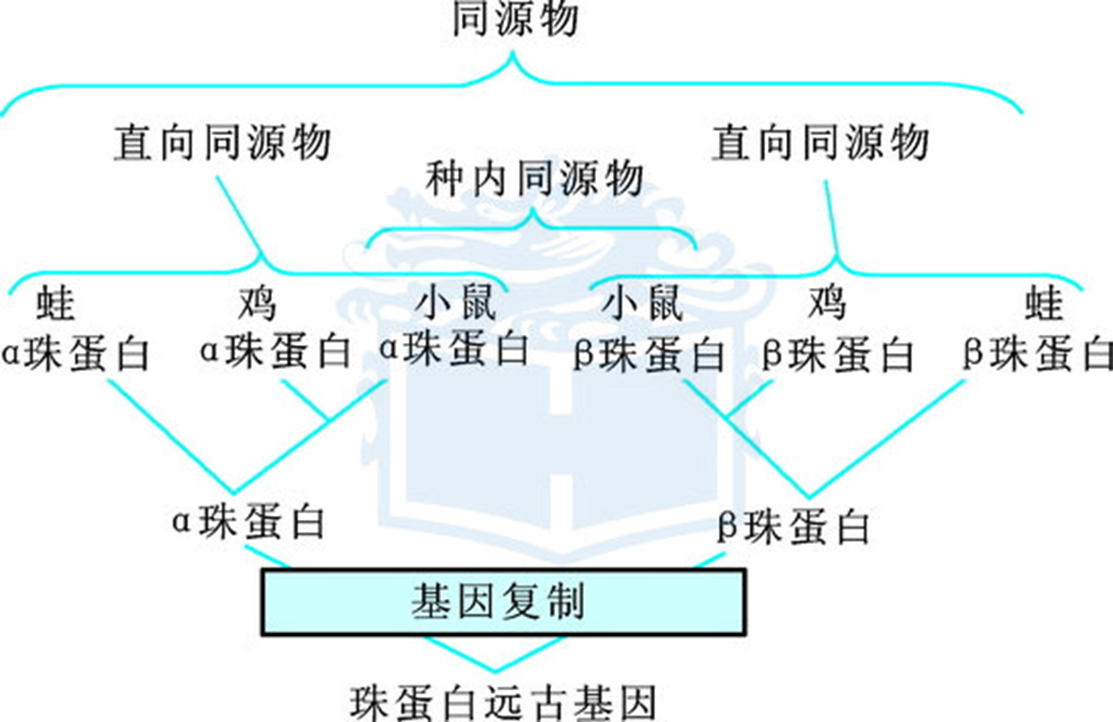
\includegraphics[width=0.7\textwidth]{三种同源关系.png}
	\caption{三种不同的同源关系}
	\label{fig:3homologs}
\end{figure}



\subsection{系统发育树}

\subsubsection{用途}

\subsubsection{结构}

根 枝 节 叶

拓扑学意义

外群 有根树 无根树

已知n个物种,最多可以建出$(2n-5)!!$棵无根树,$(2n-3)!!$棵有根树。



有根树反映进化的时间顺序

无根树只反映分类单元之间的距离

外群不太远,在分析的类群之外

\subsubsection{信息来源}

DNA?蛋白质?

\begin{itemize}
	\item 如果这一组DNA序列两两序列一致度 $>$ 70\% 那么就用DNA序;
	\item 如果这一组DNA序列两两序列一致度 $<$ 70\% 那么就用他们对应的蛋白质序列。
	\item 在实际工作中,绝大多数情况是使用蛋白质序列。
\end{itemize}

因为DNA序列一致度很高,那没必要建树

\subsubsection{算法和软件}

UPGMA NJ MP \textbf{ML} Bayesian


\section{蛋白质结构预测}

\subsection{实验法}

X射线衍射法、核磁共振法、冷冻电镜法

\subsection{软件法}

\subsubsection{二级结构预测}

PSIPRED、Jpred、APSSP2、NNPREDICT、PREDICTPROTEIN

\subsubsection{分子结构查看器}

VMD



\subsubsection{蛋白质三级结构预测}

可按照下列流程选取预测程序:(\autoref{fig:蛋白质三级结构预测程序选择})

\begin{figure}[htbp]
	\centering
	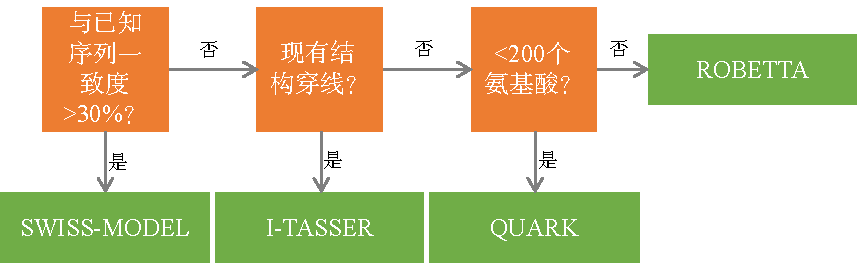
\includegraphics{蛋白质三级结构预测程序选择.pdf}
	\caption{蛋白质三级结构预测程序选择}
	\label{fig:蛋白质三级结构预测程序选择}
\end{figure}
